% =============================================================================
% The Programming Crisis of Under-Specified Compute:
% Why Traditional Compilation Fails and What Comes Next
% =============================================================================
% Single-file LaTeX with TikZ/PGFPlots only (no external images)
% =============================================================================

\documentclass[11pt,a4paper]{article}

% =============================================================================
% PREAMBLE
% =============================================================================

% ---------- Encoding & Fonts ----------
\usepackage[utf8]{inputenc}
\usepackage[T1]{fontenc}
\usepackage{lmodern}
\usepackage{microtype}

% ---------- Page Layout ----------
\usepackage[margin=1in]{geometry}
\usepackage{setspace}
\onehalfspacing

% ---------- Math ----------
\usepackage{amsmath,amssymb,amsthm}
\usepackage{mathtools}
\usepackage{bm}

% ---------- Graphics & Plotting ----------
\usepackage{tikz}
\usepackage{pgfplots}
\pgfplotsset{compat=1.18}
\usetikzlibrary{
    arrows.meta,
    positioning,
    shapes.geometric,
    shapes.misc,
    calc,
    decorations.pathreplacing,
    decorations.pathmorphing,
    patterns,
    backgrounds,
    fit,
    matrix,
    chains,
    shadows.blur
}

% ---------- Tables & Lists ----------
\usepackage{booktabs}
\usepackage{multirow}
\usepackage{enumitem}

% ---------- Colors ----------
\usepackage{xcolor}
\definecolor{codeblue}{RGB}{0,102,204}
\definecolor{codepurple}{RGB}{128,0,128}
\definecolor{codegreen}{RGB}{0,128,0}
\definecolor{codeorange}{RGB}{255,128,0}
\definecolor{lightgray}{RGB}{245,245,245}
\definecolor{darkgray}{RGB}{64,64,64}
\definecolor{accentred}{RGB}{192,0,48}
\definecolor{accentteal}{RGB}{0,128,128}

% ---------- Code Listings ----------
\usepackage{listings}
\lstset{
    basicstyle=\ttfamily\small,
    keywordstyle=\color{codeblue}\bfseries,
    commentstyle=\color{codegreen}\itshape,
    stringstyle=\color{codeorange},
    backgroundcolor=\color{lightgray},
    frame=single,
    framerule=0pt,
    breaklines=true,
    captionpos=b,
    numbers=left,
    numberstyle=\tiny\color{darkgray},
    tabsize=2
}

% ---------- Algorithms ----------
\usepackage{algorithm}
\usepackage{algpseudocode}

% ---------- References ----------
\usepackage[hidelinks]{hyperref}
\usepackage{cleveref}

% ---------- Theorems ----------
\newtheorem{theorem}{Theorem}[section]
\newtheorem{lemma}[theorem]{Lemma}
\newtheorem{proposition}[theorem]{Proposition}
\newtheorem{corollary}[theorem]{Corollary}
\newtheorem{definition}[theorem]{Definition}
\newtheorem{remark}[theorem]{Remark}
\theoremstyle{definition}
\newtheorem{example}[theorem]{Example}

% ---------- Custom Commands ----------
\newcommand{\Oh}{\mathcal{O}}
\newcommand{\E}{\mathbb{E}}
\newcommand{\R}{\mathbb{R}}
\newcommand{\N}{\mathbb{N}}
\newcommand{\vocab}{\mathcal{V}}
\newcommand{\grammar}{\mathcal{G}}

% =============================================================================
% DOCUMENT
% =============================================================================

\begin{document}

% ---------- Title ----------
\title{%
    \textbf{The Programming Crisis of Under-Specified Compute:}\\[0.3em]
    \large Why Traditional Compilation Fails and What Comes Next%
}

\author{
    David H.\ Silver\\[0.3em]
    \normalsize Kernel Keys LLC\\
    \normalsize\texttt{david@remiza.ai}
}

\date{\today}

\maketitle

% ---------- Abstract ----------
\begin{abstract}
\noindent
The computing landscape is shifting toward architectures whose functional behavior cannot be fully specified by deterministic instruction sets. Analog circuits, neuromorphic processors, optical computers, quantum devices, approximate arithmetic units, and stochastic logic all exhibit \emph{under-specified} semantics: their output depends on manufacturing variability, environmental conditions, device-specific calibration, or intrinsic randomness. Traditional compilation—which assumes a deterministic mapping from program to execution—fundamentally breaks down for such architectures. We analyze why existing approaches (manual tuning, lookup tables, simulation) fail to scale, and argue that a new paradigm is required: \emph{hardware-in-the-loop optimization} where language models generate candidate programs and configurations that are evaluated on physical hardware, with telemetry guiding iterative refinement. We present a framework for closed-loop optimization of hybrid compute systems and demonstrate its application to distributed artificial neuron nodes in robotic systems. This work establishes the theoretical and practical foundations for programming the next generation of computing substrates.
\end{abstract}

\vspace{1em}
\noindent\textbf{Keywords:} under-specified compute, hybrid architectures, hardware-in-the-loop optimization, analog computing, neuromorphic computing, optical computing, quantum computing, approximate computing, language models, robotic systems

% =============================================================================
\section{Introduction: The End of Determinism}
\label{sec:intro}
% =============================================================================

For seven decades, the dominant paradigm of computing has been \emph{determinism}: given a program and input, the output is uniquely determined. This assumption underlies every compiler, every programming language, every verification tool. Yet this paradigm is breaking down.

A new class of computing architectures is emerging—analog neural networks, neuromorphic processors, optical computers, quantum devices, approximate arithmetic units, stochastic logic gates—whose behavior is \emph{under-specified} by design. Their output depends on:
\begin{itemize}[noitemsep]
    \item Manufacturing variability (component tolerances, process variation)
    \item Environmental conditions (temperature, supply voltage, aging)
    \item Device-specific calibration (per-chip synaptic weights, optical path alignment)
    \item Intrinsic randomness (quantum measurement, stochastic switching)
\end{itemize}

These architectures offer compelling advantages: orders-of-magnitude energy efficiency, massive parallelism, compact form factors. But they present a fundamental barrier: \emph{How do you program something whose behavior you cannot fully specify?}

This paper makes three contributions:

\begin{enumerate}[noitemsep]
    \item \textbf{Crisis Analysis:} We catalog the failure modes of traditional compilation for under-specified architectures, demonstrating why deterministic abstractions break down (\Cref{sec:crisis}).
    \item \textbf{Architectural Survey:} We analyze six classes of under-specified compute (analog, neuromorphic, optical, quantum, approximate, stochastic), identifying common programming challenges (\Cref{sec:architectures}).
    \item \textbf{New Paradigm:} We propose hardware-in-the-loop optimization with language model-driven generation, establishing theoretical foundations and demonstrating application to distributed robotic systems (\Cref{sec:paradigm}).
\end{enumerate}

\Cref{fig:timeline} positions this work in the historical arc of computing abstraction.

% ---------- Figure 1: Computing Landscape ----------
\begin{figure*}[t]
\centering
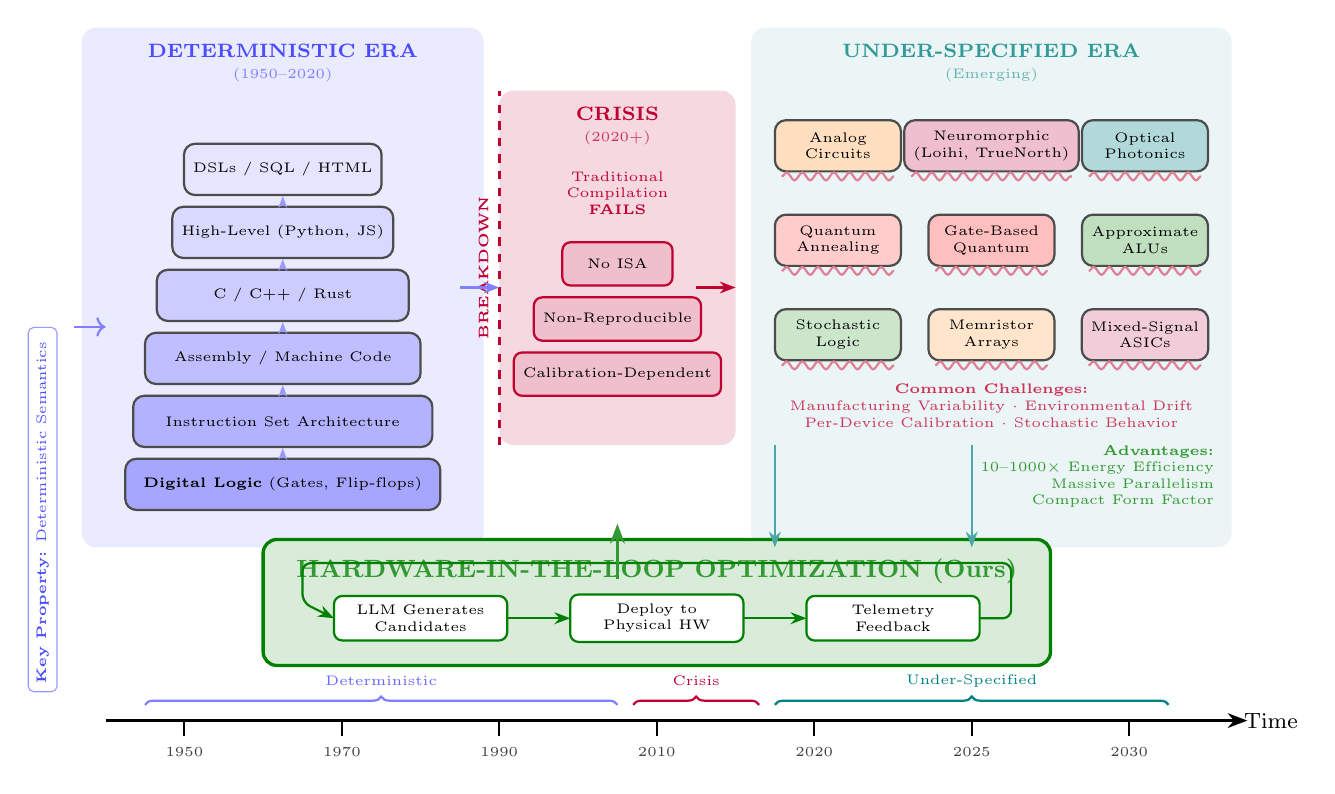
\begin{tikzpicture}[
    x=1cm, y=1cm,
    arch/.style={
        rectangle, rounded corners=4pt, draw=black!70, thick,
        minimum width=1.6cm, minimum height=0.65cm,
        align=center, font=\tiny
    },
    era/.style={
        rectangle, rounded corners=3pt, draw, thick,
        minimum width=1.4cm, minimum height=0.55cm,
        align=center, font=\tiny
    }
]

% === LEFT PANEL: Deterministic Stack (Historical) ===
\begin{scope}
    % Background
    \fill[blue!8, rounded corners=5pt] (-0.3, -0.3) rectangle (4.8, 6.3);
    \node[font=\scriptsize\bfseries, text=blue!70] at (2.25, 6) {DETERMINISTIC ERA};
    \node[font=\tiny, text=blue!50] at (2.25, 5.7) {(1950--2020)};
    
    % Stack layers (bottom to top)
    \node[arch, fill=blue!35, minimum width=4cm] (hw) at (2.25, 0.5) {\textbf{Digital Logic} (Gates, Flip-flops)};
    \node[arch, fill=blue!30, minimum width=3.8cm] (isa) at (2.25, 1.3) {Instruction Set Architecture};
    \node[arch, fill=blue!25, minimum width=3.5cm] (asm) at (2.25, 2.1) {Assembly / Machine Code};
    \node[arch, fill=blue!20, minimum width=3.2cm] (c) at (2.25, 2.9) {C / C++ / Rust};
    \node[arch, fill=blue!15, minimum width=2.8cm] (hl) at (2.25, 3.7) {High-Level (Python, JS)};
    \node[arch, fill=blue!10, minimum width=2.4cm] (dsl) at (2.25, 4.5) {DSLs / SQL / HTML};
    
    % Arrows between layers
    \foreach \a/\b in {hw/isa, isa/asm, asm/c, c/hl, hl/dsl} {
        \draw[-{Stealth[length=1.5mm]}, blue!40, thick] (\a) -- (\b);
    }
    
\end{scope}

% === CENTER: THE CRISIS ===
\begin{scope}[xshift=5.5cm]
    % Crisis zone background
    \fill[accentred!15, rounded corners=5pt] (-0.5, 1) rectangle (2.5, 5.5);
    \draw[accentred, very thick, dashed, rounded corners=5pt] (-0.5, 1) -- (-0.5, 5.5);
    
    \node[font=\scriptsize\bfseries, text=accentred] at (1, 5.2) {CRISIS};
    \node[font=\tiny, text=accentred!80] at (1, 4.9) {(2020+)};
    
    % Problem statements
    \node[font=\tiny, text=accentred, align=center] at (1, 4.2) {%
        Traditional\\
        Compilation\\
        \textbf{FAILS}
    };
    
    % Failure modes (stacked)
    \node[era, fill=accentred!25, draw=accentred] at (1, 3.3) {No ISA};
    \node[era, fill=accentred!25, draw=accentred] at (1, 2.6) {Non-Reproducible};
    \node[era, fill=accentred!25, draw=accentred] at (1, 1.9) {Calibration-Dependent};
    
    % Arrow showing breakdown
    \node[font=\tiny, accentred, rotate=90] at (-0.7, 3.25) {\textbf{BREAKDOWN}};
\end{scope}

% === RIGHT PANEL: Under-Specified Architectures ===
\begin{scope}[xshift=8.5cm]
    % Background
    \fill[accentteal!8, rounded corners=5pt] (-0.3, -0.3) rectangle (5.8, 6.3);
    \node[font=\scriptsize\bfseries, text=accentteal!80] at (2.75, 6) {UNDER-SPECIFIED ERA};
    \node[font=\tiny, text=accentteal!60] at (2.75, 5.7) {(Emerging)};
    
    % 2x3 Grid of architecture classes
    % Row 1
    \node[arch, fill=orange!25] (analog) at (0.8, 4.8) {Analog\\Circuits};
    \node[arch, fill=purple!25] (neuro) at (2.75, 4.8) {Neuromorphic\\(Loihi, TrueNorth)};
    \node[arch, fill=accentteal!30] (optical) at (4.7, 4.8) {Optical\\Photonics};
    
    % Row 2
    \node[arch, fill=red!20] (quantum) at (0.8, 3.6) {Quantum\\Annealing};
    \node[arch, fill=red!25] (qgate) at (2.75, 3.6) {Gate-Based\\Quantum};
    \node[arch, fill=codegreen!25] (approx) at (4.7, 3.6) {Approximate\\ALUs};
    
    % Row 3
    \node[arch, fill=codegreen!20] (stoch) at (0.8, 2.4) {Stochastic\\Logic};
    \node[arch, fill=orange!20] (memristor) at (2.75, 2.4) {Memristor\\Arrays};
    \node[arch, fill=purple!20] (mixsig) at (4.7, 2.4) {Mixed-Signal\\ASICs};
    
    % Variability indicators (wavy underlines)
    \foreach \node in {analog, neuro, optical, quantum, qgate, approx, stoch, memristor, mixsig} {
        \draw[accentred!50, thick, decorate, decoration={snake, amplitude=0.5mm, segment length=2mm}] 
            ($(\node.south west) + (0.1, -0.05)$) -- ($(\node.south east) + (-0.1, -0.05)$);
    }
    
    % Common challenges box
    \node[font=\tiny, text=accentred!80, align=center] at (2.75, 1.5) {%
        \textbf{Common Challenges:}\\
        Manufacturing Variability $\cdot$ Environmental Drift\\
        Per-Device Calibration $\cdot$ Stochastic Behavior
    };
    
    % Efficiency annotation
    \node[font=\tiny, text=codegreen!80, align=right, anchor=east] at (5.7, 0.6) {%
        \textbf{Advantages:}\\
        10--1000$\times$ Energy Efficiency\\
        Massive Parallelism\\
        Compact Form Factor
    };
\end{scope}

% === BOTTOM: OUR SOLUTION ===
\begin{scope}[yshift=-1.5cm]
    % Solution box (spans full width)
    \fill[codegreen!15, rounded corners=5pt] (2, -0.3) rectangle (12, 1.3);
    \draw[codegreen, very thick, rounded corners=5pt] (2, -0.3) rectangle (12, 1.3);
    
    \node[font=\small\bfseries, text=codegreen!80] at (7, 0.9) {HARDWARE-IN-THE-LOOP OPTIMIZATION (Ours)};
    
    % Three components
    \node[era, fill=white, draw=codegreen, minimum width=2.2cm] at (4, 0.3) {LLM Generates\\Candidates};
    \node[era, fill=white, draw=codegreen, minimum width=2.2cm] at (7, 0.3) {Deploy to\\Physical HW};
    \node[era, fill=white, draw=codegreen, minimum width=2.2cm] at (10, 0.3) {Telemetry\\Feedback};
    
    % Cycle arrows
    \draw[-{Stealth[length=2mm]}, codegreen, thick] (5.1, 0.3) -- (5.9, 0.3);
    \draw[-{Stealth[length=2mm]}, codegreen, thick] (8.1, 0.3) -- (8.9, 0.3);
    \draw[-{Stealth[length=2mm]}, codegreen, thick, rounded corners=3pt] (11.1, 0.3) -- (11.5, 0.3) -- (11.5, 1) -- (2.5, 1) -- (2.5, 0.5) -- (2.9, 0.3);
    
    % Arrows from crisis to solution
    \draw[-{Stealth[length=2.5mm]}, codegreen!80, very thick] (6.5, 0.8) -- (6.5, 1.5);
\end{scope}

% === CONNECTING ARROWS ===
% From deterministic to crisis
\draw[-{Stealth[length=2mm]}, blue!50, thick] (4.5, 3) -- (5, 3);

% From crisis to under-specified
\draw[-{Stealth[length=2mm]}, accentred, thick] (7.5, 3) -- (8, 3);

% From under-specified to solution
\draw[-{Stealth[length=2mm]}, accentteal!70, thick] (11, 1) -- (11, -0.3);
\draw[-{Stealth[length=2mm]}, accentteal!70, thick] (8.5, 1) -- (8.5, -0.3);

% Time axis
\draw[thick, -{Stealth[length=2.5mm]}] (0, -2.5) -- (14.5, -2.5);
\node[font=\footnotesize] at (14.8, -2.5) {Time};
\foreach \x/\yr in {1/1950, 3/1970, 5/1990, 7/2010, 9/2020, 11/2025, 13/2030} {
    \draw[thick] (\x, -2.5) -- (\x, -2.7);
    \node[font=\tiny, text=darkgray] at (\x, -2.9) {\yr};
}

% Era brackets on timeline
\draw[blue!50, thick, decorate, decoration={brace, amplitude=3pt}] (0.5, -2.3) -- (6.5, -2.3);
\node[font=\tiny, text=blue!60] at (3.5, -2) {Deterministic};

\draw[accentred, thick, decorate, decoration={brace, amplitude=3pt}] (6.7, -2.3) -- (8.3, -2.3);
\node[font=\tiny, text=accentred] at (7.5, -2) {Crisis};

\draw[accentteal, thick, decorate, decoration={brace, amplitude=3pt}] (8.5, -2.3) -- (13.5, -2.3);
\node[font=\tiny, text=accentteal] at (11, -2) {Under-Specified};

% === TOP LAYER: Key Property annotation (positioned left of stack, vertically centered) ===
\node[font=\tiny, text=blue!70, align=center, anchor=east, 
      fill=white, draw=blue!40, rounded corners=2pt, inner sep=3pt, rotate=90] at (-0.8, 2.5) {%
    \textbf{Key Property:} Deterministic Semantics
};
\draw[blue!50, thick, ->] (-0.4, 2.5) -- (0.0, 2.5);

\end{tikzpicture}
\caption{The computing landscape: determinism vs.\ under-specification. \textbf{Left:} The deterministic era (1950--2020) built stable abstraction layers from digital logic to high-level languages, all assuming reproducible semantics. \textbf{Center:} Emerging under-specified architectures (analog, neuromorphic, optical, quantum, approximate, stochastic) break this assumption---they have no ISA, exhibit manufacturing variability, and require per-device calibration. Traditional compilation fails. \textbf{Right:} These architectures offer compelling efficiency advantages but create a programming crisis. \textbf{Bottom:} Hardware-in-the-loop optimization (our paradigm) resolves this by optimizing directly on physical hardware with LLM-driven generation and telemetry feedback.}
\label{fig:timeline}
\end{figure*}

% =============================================================================
\section{The Programming Crisis: Why Traditional Compilation Fails}
\label{sec:crisis}
% =============================================================================

Traditional compilation assumes a \emph{deterministic instruction set architecture} (ISA): given an instruction and state, the next state is uniquely determined. This assumption underlies:

\begin{itemize}[noitemsep]
    \item \textbf{Syntax-directed translation:} Grammar rules map to deterministic code generation
    \item \textbf{Optimization passes:} Transformations preserve program semantics
    \item \textbf{Verification:} Model checking and theorem proving assume deterministic transitions
    \item \textbf{Debugging:} Reproducible execution enables systematic error isolation
\end{itemize}

When hardware behavior is under-specified, these foundations crumble.

\subsection{The Specification Gap}

\begin{definition}[Under-Specified Compute Element]
An under-specified compute element is one whose functional mapping $f: \mathcal{I} \to \mathcal{O}$ cannot be fully specified by a deterministic program. Instead, the mapping depends on:
\begin{itemize}[noitemsep]
    \item A set of \emph{configuration parameters} $\theta \in \Theta$ (calibration, weights, routing)
    \item \emph{Environmental state} $e \in \mathcal{E}$ (temperature, voltage, aging)
    \item \emph{Manufacturing variability} $v \in \mathcal{V}$ (component tolerances, process variation)
    \item Potentially \emph{stochastic behavior} $s \sim \mathcal{S}$
\end{itemize}
The effective mapping is $f_{\theta,e,v,s}: \mathcal{I} \to \mathcal{O}$, where $\theta$, $e$, $v$, and $s$ are not fully known or controllable.
\end{definition}

\subsection{Failure Mode 1: Non-Reproducible Execution}

Traditional debugging relies on reproducibility: run the same program with the same input, observe the same output. Under-specified architectures violate this:

\begin{example}[Analog Neural Network]
An analog neural network computes $y = \sigma(Wx + b)$ where $W$ and $b$ are implemented as resistor values. Manufacturing tolerances cause $W_{ij}$ to vary by $\pm 5\%$ across chips. Running the ``same'' program on two chips produces different outputs. Traditional debugging—which assumes deterministic execution—cannot isolate whether differences are due to bugs or manufacturing variation.
\end{example}

\subsection{Failure Mode 2: Environment-Dependent Semantics}

Program behavior changes with environmental conditions:

\begin{example}[Optical Computing]
An optical matrix multiplier uses interferometric paths. The effective matrix $M$ depends on:
\begin{itemize}[noitemsep]
    \item Temperature (thermal expansion changes path lengths)
    \item Mechanical vibration (alignment drift)
    \item Aging (material degradation)
\end{itemize}
A program that works at 20$^\circ$C may fail at 40$^\circ$C. Traditional compilation assumes environment-independent semantics.
\end{example}

\subsection{Failure Mode 3: Calibration-Dependent Correctness}

Correctness depends on per-device calibration:

\begin{example}[Neuromorphic Processor]
A neuromorphic chip implements synaptic weights as memristor conductances. Each chip requires per-device calibration to map desired weights to actual conductances. The ``program'' (weight matrix) is meaningless without calibration data. Traditional compilers cannot generate calibration-dependent code.
\end{example}

\subsection{Failure Mode 4: Stochastic Semantics}

Some architectures intentionally randomize behavior:

\begin{example}[Stochastic Computing]
A stochastic adder computes $z = x + y$ by sampling random bitstreams. The output is correct \emph{in expectation} but varies across runs. Traditional verification (which checks exact correctness) fails; probabilistic verification is required.
\end{example}

\subsection{Failure Mode 5: Approximate Correctness}

Approximate architectures trade exactness for efficiency:

\begin{example}[Approximate Multipliers]
An approximate multiplier may compute $z \approx x \times y$ with $95\%$ accuracy. Traditional compilers assume exact arithmetic; approximate semantics require new type systems and verification methods.
\end{example}

\subsection{Why Existing Approaches Fail}

\paragraph{Manual Tuning.} Hardware experts manually calibrate each device. This does not scale: deploying to 10,000 devices requires 10,000 expert-hours. Moreover, manual tuning cannot discover optimal configurations—experts rely on heuristics and intuition. For a device with $d$ calibration parameters, the search space has $|\Theta|^d$ configurations. Even with $|\Theta| = 10$ and $d = 20$, this is $10^{20}$ configurations—intractable for manual exploration.

\paragraph{Lookup Tables.} Pre-characterize devices and store input-output mappings. This is inflexible: new programs require new characterization, and tables grow exponentially with input dimension. For an $n$-bit input, a complete lookup table requires $2^n$ entries. For $n=32$, this is $4.3 \times 10^9$ entries—4.3 GB per table. For multi-input functions, the curse of dimensionality makes this approach intractable. Moreover, lookup tables cannot generalize: if a new input appears that was not in the characterization set, the system fails.

\paragraph{Monte Carlo Simulation.} Simulate device behavior with variability models. This is slow (millions of samples) and may not capture real hardware behavior (models are imperfect). To estimate output variance with confidence $\delta$ and error $\epsilon$, Monte Carlo requires $N = \Oh(1/\epsilon^2 \log(1/\delta))$ samples. For $\epsilon = 0.01$ and $\delta = 0.05$, this is $N \approx 40,000$ samples per input. For a program with $10^6$ inputs, this requires $4 \times 10^{10}$ simulations—computationally prohibitive. Worse, simulation models are abstractions: they omit second-order effects (crosstalk, substrate coupling, quantum effects) that affect real hardware.

\paragraph{Exhaustive Characterization.} Measure all input-output pairs. This is intractable: for a 32-bit input, $2^{32}$ measurements are required. At 1 ms per measurement, this requires 50 days of continuous measurement per device. For multi-input functions or continuous inputs, exhaustive characterization is impossible. Moreover, characterization must be repeated for each device (manufacturing variation) and each environmental condition (temperature, voltage), making the approach fundamentally unscalable.

\paragraph{Deterministic Abstraction.} Ignore variability and assume deterministic behavior. This leads to brittle programs that fail in production. The abstraction gap between assumed behavior (deterministic) and actual behavior (variable) causes:
\begin{itemize}[noitemsep]
    \item \textbf{Silent failures:} Programs produce wrong outputs without error signals
    \item \textbf{Intermittent bugs:} Failures occur only under certain environmental conditions
    \item \textbf{Non-portability:} Programs work on one device but fail on another (manufacturing variation)
    \item \textbf{Safety violations:} In safety-critical systems, abstraction gaps can cause catastrophic failures
\end{itemize}

\subsection{The Compiler's Dilemma}

Traditional compilers face a fundamental dilemma when targeting under-specified hardware:

\begin{enumerate}[noitemsep]
    \item \textbf{If they ignore variability:} Generated code is brittle and fails in production
    \item \textbf{If they model variability:} They must solve an intractable optimization problem (find configuration $\theta$ that works across all devices and environments)
    \item \textbf{If they require per-device calibration:} They cannot generate code offline—calibration must happen at deployment time
\end{enumerate}

This dilemma has no solution within the traditional compilation framework. A new paradigm is required.

\subsection{Complexity Analysis}

We formalize why traditional compilation fails through complexity analysis:

\begin{theorem}[Intractability of Deterministic Compilation]
\label{thm:intractability}
For an under-specified compute element with $d$ configuration parameters, $m$ devices (manufacturing variation), and $e$ environmental conditions, finding a single configuration that works for all devices and environments requires solving:
\[
\min_{\theta} \max_{v \in \mathcal{V}, e \in \mathcal{E}} \text{Error}(f_{\theta,v,e}, f_{\text{desired}})
\]
This is a minimax optimization over $|\mathcal{V}| \times |\mathcal{E}|$ constraints. For $|\mathcal{V}| = 10^3$ devices and $|\mathcal{E}| = 10^2$ conditions, this is $10^5$ constraints—intractable for traditional optimization.
\end{theorem}

\begin{proof}[Proof sketch]
Traditional compilers use deterministic optimization (gradient descent, branch-and-bound). Minimax optimization over discrete sets $\mathcal{V}$ and $\mathcal{E}$ is NP-hard. Even approximation requires exponential time in the worst case.
\end{proof}

\subsection{The Verification Crisis}

Traditional verification assumes deterministic semantics. Under-specified architectures require probabilistic verification:

\begin{proposition}[Verification Complexity]
\label{prop:verification}
Verifying that an under-specified program satisfies a property $P$ with confidence $1-\delta$ requires:
\begin{itemize}[noitemsep]
    \item \textbf{Deterministic verification:} $\Oh(|\text{state space}|)$ (exponential in program size)
    \item \textbf{Probabilistic verification:} $\Oh(1/\epsilon^2 \log(1/\delta))$ samples per device-environment pair
\end{itemize}
For $m$ devices and $e$ environments, probabilistic verification requires $m \times e \times \Oh(1/\epsilon^2 \log(1/\delta))$ samples—prohibitive for large deployments.
\end{proposition}

\Cref{fig:failure_modes} illustrates these failure modes.

% ---------- Figure 2: Failure Modes ----------
\begin{figure}[t]
\centering
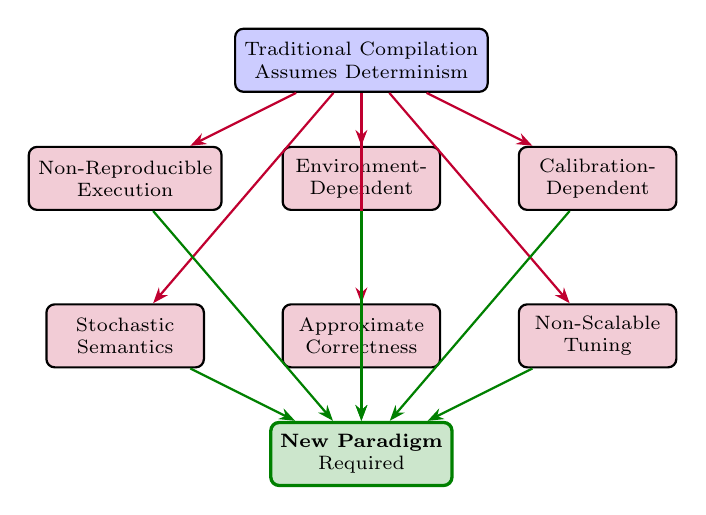
\begin{tikzpicture}[
    x=1cm, y=1cm,
    box/.style={
        rectangle, rounded corners=3pt, draw, thick,
        minimum width=2cm, minimum height=0.8cm,
        align=center, font=\scriptsize
    },
    arrow/.style={-{Stealth[length=2mm]}, thick}
]

% Traditional compilation
\node[box, fill=blue!20] (traditional) at (5, 5) {Traditional Compilation\\Assumes Determinism};

% Failure modes (radiating out)
\node[box, fill=accentred!20] (nonrep) at (2, 3.5) {Non-Reproducible\\Execution};
\node[box, fill=accentred!20] (env) at (5, 3.5) {Environment-\\Dependent};
\node[box, fill=accentred!20] (calib) at (8, 3.5) {Calibration-\\Dependent};
\node[box, fill=accentred!20] (stoch) at (2, 1.5) {Stochastic\\Semantics};
\node[box, fill=accentred!20] (approx) at (5, 1.5) {Approximate\\Correctness};
\node[box, fill=accentred!20] (scale) at (8, 1.5) {Non-Scalable\\Tuning};

% Arrows
\draw[arrow, accentred] (traditional) -- (nonrep);
\draw[arrow, accentred] (traditional) -- (env);
\draw[arrow, accentred] (traditional) -- (calib);
\draw[arrow, accentred] (traditional) -- (stoch);
\draw[arrow, accentred] (traditional) -- (approx);
\draw[arrow, accentred] (traditional) -- (scale);

% Result
\node[box, fill=codegreen!20, draw=codegreen, very thick] (solution) at (5, 0) {\textbf{New Paradigm}\\Required};

\draw[arrow, codegreen, thick] (nonrep) -- (solution);
\draw[arrow, codegreen, thick] (env) -- (solution);
\draw[arrow, codegreen, thick] (calib) -- (solution);
\draw[arrow, codegreen, thick] (stoch) -- (solution);
\draw[arrow, codegreen, thick] (approx) -- (solution);
\draw[arrow, codegreen, thick] (scale) -- (solution);

\end{tikzpicture}
\caption{Failure modes of traditional compilation for under-specified architectures. All paths lead to the conclusion that a new paradigm is required.}
\label{fig:failure_modes}
\end{figure}

% =============================================================================
\section{Architectural Survey: Six Classes of Under-Specified Compute}
\label{sec:architectures}
% =============================================================================

We analyze six classes of under-specified compute, identifying common programming challenges.

\subsection{Analog and Mixed-Signal Circuits}

Analog circuits compute with continuous voltages and currents. Examples include:
\begin{itemize}[noitemsep]
    \item \textbf{Analog neural networks:} Matrix-vector multiplication via resistor networks
    \item \textbf{Analog filters:} Signal processing with RC/LC circuits
    \item \textbf{Analog-to-digital converters:} Quantization with comparator arrays
    \item \textbf{Phase-locked loops:} Frequency synthesis and clock recovery
\end{itemize}

\paragraph{Programming Challenges.}
\begin{itemize}[noitemsep]
    \item Component tolerances ($\pm 5\%$ resistors, $\pm 10\%$ capacitors) cause output variation
    \item Temperature coefficients ($\sim 100$ ppm/$^\circ$C) shift behavior
    \item Supply voltage sensitivity (rail-to-rail operation depends on $V_{DD}$)
    \item Aging effects (drift over time)
\end{itemize}

\paragraph{Why Traditional Compilation Fails.}
Compilers assume digital semantics (0/1, exact arithmetic). Analog circuits have continuous, noisy, temperature-dependent behavior. There is no ``instruction set''—only component values and topologies.

Consider compiling a neural network layer $y = \text{ReLU}(Wx + b)$ to an analog circuit. The compiler must:
\begin{enumerate}[noitemsep]
    \item Map matrix $W$ to resistor values $R_{ij}$ (Ohm's law: $V = IR$)
    \item Account for manufacturing tolerances: $R_{ij} = R_{\text{nominal}} \times (1 + \epsilon_{ij})$ where $\epsilon_{ij} \sim \mathcal{N}(0, \sigma^2)$
    \item Compensate for temperature drift: $R(T) = R(T_0) \times (1 + \alpha(T - T_0))$ where $\alpha \approx 100$ ppm/$^\circ$C
    \item Handle supply voltage variation: $V_{out} = f(V_{in}, V_{DD})$ where $V_{DD}$ varies $\pm 5\%$
\end{enumerate}

Traditional compilers cannot handle this: they generate discrete instructions, not continuous component values. Even if they could, the optimization problem (find $R_{ij}$ that work across all temperatures, voltages, and manufacturing variations) is intractable.

\paragraph{Case Study: Analog Matrix Multiplier.}
An analog matrix multiplier computes $y = Mx$ using resistor networks. For a $64 \times 64$ matrix, this requires $4,096$ resistors. Manufacturing tolerances cause each resistor to vary by $\pm 5\%$. The output error is:
\[
\epsilon_{\text{output}} = \sum_{i,j} \frac{\partial y_i}{\partial M_{ij}} \epsilon_{M_{ij}}
\]
where $\epsilon_{M_{ij}}$ is the resistor tolerance. For worst-case tolerance accumulation, $\epsilon_{\text{output}}$ can exceed $50\%$—unacceptable for most applications. Traditional compilers cannot generate error-correcting code for analog circuits; the errors are physical, not logical.

\subsection{Neuromorphic and Spiking Circuits}

Neuromorphic processors mimic biological neurons with:
\begin{itemize}[noitemsep]
    \item \textbf{Memristor synapses:} Programmable conductances
    \item \textbf{Spike-based communication:} Event-driven signaling
    \item \textbf{Leaky integrate-and-fire neurons:} Temporal dynamics
\end{itemize}

Examples: Intel Loihi, IBM TrueNorth, SpiNNaker.

\paragraph{Programming Challenges.}
\begin{itemize}[noitemsep]
    \item Device-to-device variability in synaptic weights (memristor $R_{on}/R_{off}$ ratio varies)
    \item Temporal dynamics (spike timing, refractory periods) are difficult to model
    \item Calibration required per chip (map desired weights to actual conductances)
    \item Stochastic behavior (probabilistic spike generation)
\end{itemize}

\paragraph{Why Traditional Compilation Fails.}
Traditional compilers generate static code. Neuromorphic systems require:
\begin{itemize}[noitemsep]
    \item Weight matrices (not instructions)
    \item Per-device calibration data
    \item Temporal event scheduling
\end{itemize}
These cannot be generated by deterministic compilation.

The fundamental challenge is \emph{device-to-device variability}. Memristor conductances vary by orders of magnitude across chips. A desired weight $w_{ij}$ must be mapped to a memristor conductance $G_{ij}$ via calibration:
\[
G_{ij} = \text{Calibrate}(w_{ij}, \text{DeviceID})
\]
This calibration is device-specific and cannot be computed offline. Traditional compilers generate code once; neuromorphic systems require per-device calibration at deployment time.

Moreover, neuromorphic systems have \emph{temporal dynamics}: spikes propagate with delays, neurons have refractory periods, synapses have temporal integration. Traditional compilers assume synchronous execution; neuromorphic systems are inherently asynchronous and event-driven. There is no ``clock''—only spike events.

\paragraph{Case Study: Intel Loihi.}
Loihi has 128,000 neurons and 128 million synapses. Each synapse is a memristor with $R_{on}/R_{off}$ ratio varying from $10^2$ to $10^6$ across devices. To program Loihi, you must:
\begin{enumerate}[noitemsep]
    \item Specify desired weight matrix $W \in \R^{128K \times 128K}$
    \item For each device, calibrate: $G_{ij} = f(W_{ij}, \text{chip-specific params})$
    \item Account for temporal dynamics: spike delays, refractory periods, synaptic integration
\end{enumerate}
Traditional compilers cannot do this: they generate instructions, not weight matrices and calibration data. Even if they could, the calibration problem (map $W$ to $G$ for each device) is a $128K \times 128K$ optimization problem—intractable.

\subsection{Optical Computing}

Optical computers use light for computation:
\begin{itemize}[noitemsep]
    \item \textbf{Optical matrix multipliers:} Interferometric matrix-vector products
    \item \textbf{Photonic neural networks:} Weighted optical paths
    \item \textbf{Optical signal processing:} Fourier transforms via lenses
    \item \textbf{Quantum photonic circuits:} Entangled photon manipulation
\end{itemize}

\paragraph{Programming Challenges.}
\begin{itemize}[noitemsep]
    \item Alignment sensitivity (micrometer-scale path differences cause errors)
    \item Thermal drift (refractive index changes with temperature)
    \item Manufacturing variation (waveguide dimensions, coupling coefficients)
    \item Loss and noise (photons are lost, detectors have noise)
\end{itemize}

\paragraph{Why Traditional Compilation Fails.}
Optical systems have no ``instructions''—only:
\begin{itemize}[noitemsep]
    \item Waveguide routing (physical layout)
    \item Phase modulators (analog control voltages)
    \item Detector thresholds (calibration-dependent)
\end{itemize}
These are physical parameters, not program code.

The challenge is \emph{alignment sensitivity}. Optical paths must be aligned to micrometer precision. A path length error of $\lambda/10$ (where $\lambda$ is wavelength) causes phase errors that corrupt computation. Thermal expansion changes path lengths by $\Delta L = L \alpha \Delta T$ where $\alpha \approx 10^{-5}$/$^\circ$C. For a 1 cm path and 20$^\circ$C temperature change, $\Delta L = 2$ $\mu$m---comparable to wavelength ($\lambda \approx 1.5$ $\mu$m for near-infrared). This makes optical systems extremely sensitive to temperature.

Traditional compilers cannot generate temperature-compensated code: the compensation depends on physical layout (which paths are long, which are short) and cannot be determined from a high-level program description.

\paragraph{Case Study: Photonic Neural Network.}
A photonic neural network implements $y = \sigma(Wx)$ using interferometric matrix multiplication. The effective weight matrix $W_{\text{effective}}$ depends on:
\begin{itemize}[noitemsep]
    \item Phase modulator settings: $W_{\text{effective}} = W_{\text{desired}} \times e^{i\phi}$ where $\phi$ is phase error
    \item Path length differences: $\phi = 2\pi \Delta L / \lambda$ where $\Delta L$ varies with temperature
    \item Coupling coefficients: vary with manufacturing (waveguide width tolerances)
\end{itemize}
To program such a system, you must solve:
\[
\min_{\phi, \text{coupling}} \|W_{\text{effective}}(\phi, \text{coupling}, T) - W_{\text{desired}}\|
\]
for all temperatures $T$ in the operating range. This is a non-convex optimization over continuous parameters with temperature-dependent constraints—intractable for traditional compilers.

\subsection{Quantum Computing}

Quantum computers exploit superposition and entanglement:
\begin{itemize}[noitemsep]
    \item \textbf{Gate-based quantum:} Unitary operations on qubits
    \item \textbf{Quantum annealing:} Adiabatic optimization
    \item \textbf{Photonic quantum:} Linear optical quantum computing
\end{itemize}

\paragraph{Programming Challenges.}
\begin{itemize}[noitemsep]
    \item Decoherence (quantum states decay)
    \item Gate errors (imperfect unitary operations)
    \item Measurement noise (detector imperfections)
    \item Calibration (per-qubit $T_1$, $T_2$, gate fidelities)
    \item Intrinsic randomness (measurement outcomes are probabilistic)
\end{itemize}

\paragraph{Why Traditional Compilation Fails.}
Quantum programs are:
\begin{itemize}[noitemsep]
    \item Probabilistic (measurement outcomes are random)
    \item Calibration-dependent (gate fidelities vary per device)
    \item Error-prone (decoherence, gate errors)
\end{itemize}
Traditional compilers assume deterministic, error-free execution.

The fundamental challenge is \emph{decoherence}: quantum states decay exponentially with time constant $T_2$. A quantum gate that takes time $\tau$ has fidelity:
\[
F = 1 - e^{-\tau/T_2}
\]
For $T_2 = 100$ $\mu$s and $\tau = 1$ $\mu$s, $F \approx 0.99$—acceptable. But $T_2$ varies across qubits (manufacturing variation) and over time (aging). A compiler that assumes fixed $T_2$ generates code that fails on some qubits.

Moreover, quantum programs are \emph{probabilistic}: measurement outcomes are random. A program that computes $f(x)$ actually computes a probability distribution $P(f(x) = y)$. Traditional compilers cannot reason about probabilistic correctness.

\paragraph{Case Study: Google Sycamore.}
Sycamore has 53 qubits with $T_2$ ranging from 10 $\mu$s to 200 $\mu$s. Gate fidelities vary from 99.3\% to 99.9\% across qubits. To compile a quantum algorithm:
\begin{enumerate}[noitemsep]
    \item Map logical qubits to physical qubits (accounting for $T_2$ and gate fidelities)
    \item Schedule gates to minimize decoherence (shorter circuits = higher fidelity)
    \item Insert error correction (but error correction itself has errors)
\end{enumerate}
This is a constrained optimization: maximize fidelity subject to connectivity constraints (not all qubits are connected). Traditional compilers use heuristics (greedy mapping, shortest-path routing) that are suboptimal. Optimal compilation is NP-hard.

\subsection{Approximate Computing}

Approximate architectures trade exactness for efficiency:
\begin{itemize}[noitemsep]
    \item \textbf{Approximate adders:} $95\%$ accuracy, $50\%$ energy
    \item \textbf{Approximate multipliers:} Truncated partial products
    \item \textbf{Voltage-scaled circuits:} Near-threshold operation
    \item \textbf{Stochastic computing:} Bitstream arithmetic
\end{itemize}

\paragraph{Programming Challenges.}
\begin{itemize}[noitemsep]
    \item Error bounds vary with input (some inputs more error-prone)
    \item Quality-energy tradeoffs (more approximation = less energy)
    \item Application-dependent tolerance (image processing vs. financial)
    \item Verification requires probabilistic analysis
\end{itemize}

\paragraph{Why Traditional Compilation Fails.}
Traditional compilers assume exact arithmetic. Approximate computing requires:
\begin{itemize}[noitemsep]
    \item Error-aware type systems
    \item Quality-energy optimization
    \item Probabilistic verification
\end{itemize}
These are not supported by standard compilation toolchains.

\subsection{Stochastic and Probabilistic Logic}

Stochastic systems intentionally randomize behavior:
\begin{itemize}[noitemsep]
    \item \textbf{Stochastic computing:} Bitstream-based arithmetic
    \item \textbf{Probabilistic logic:} Random switching for security
    \item \textbf{Monte Carlo methods:} Randomized algorithms
\end{itemize}

\paragraph{Programming Challenges.}
\begin{itemize}[noitemsep]
    \item Correctness is probabilistic (correct in expectation, not exactly)
    \item Variance depends on sequence length (longer = lower variance)
    \item Verification requires statistical analysis
    \item Debugging is difficult (non-reproducible execution)
\end{itemize}

\paragraph{Why Traditional Compilation Fails.}
Traditional compilers generate deterministic code. Stochastic systems require:
\begin{itemize}[noitemsep]
    \item Random number generation (hardware RNGs)
    \item Statistical correctness (not exact)
    \item Variance analysis
\end{itemize}
These cannot be handled by deterministic compilation.

\Cref{fig:architectures} summarizes the six classes and their common challenges.

% ---------- Figure 3: Architecture Classes ----------
\begin{figure}[t]
\centering
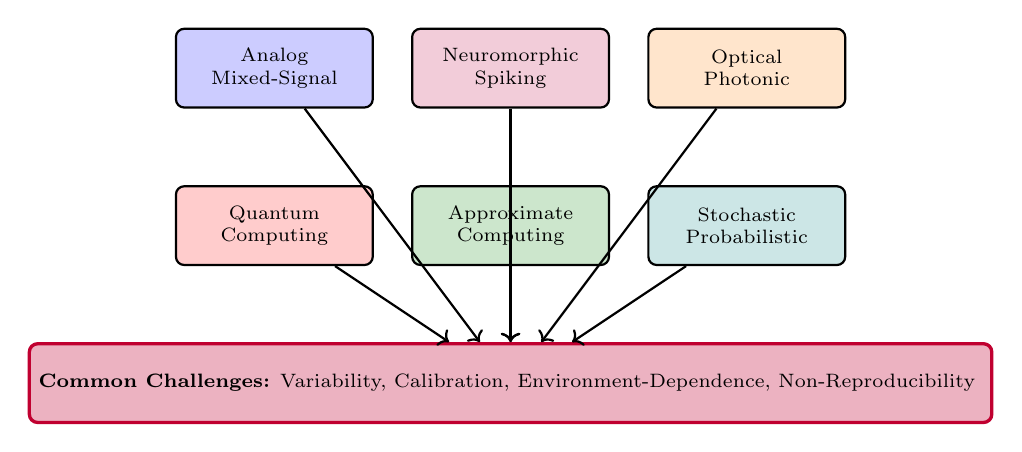
\begin{tikzpicture}[
    x=1cm, y=1cm,
    arch/.style={
        rectangle, rounded corners=3pt, draw, thick,
        minimum width=2.5cm, minimum height=1cm,
        align=center, font=\scriptsize
    }
]

% Six classes arranged in 2x3 grid
\node[arch, fill=blue!20] (analog) at (2, 4.5) {Analog\\Mixed-Signal};
\node[arch, fill=purple!20] (neuro) at (5, 4.5) {Neuromorphic\\Spiking};
\node[arch, fill=orange!20] (optical) at (8, 4.5) {Optical\\Photonic};

\node[arch, fill=red!20] (quantum) at (2, 2.5) {Quantum\\Computing};
\node[arch, fill=codegreen!20] (approx) at (5, 2.5) {Approximate\\Computing};
\node[arch, fill=accentteal!20] (stoch) at (8, 2.5) {Stochastic\\Probabilistic};

% Common challenges (bottom)
\node[arch, fill=accentred!30, draw=accentred, very thick, minimum width=8cm] (challenges) at (5, 0.5) {
    \textbf{Common Challenges:} Variability, Calibration, Environment-Dependence, Non-Reproducibility
};

% Arrows
\draw[->, thick] (analog) -- (challenges);
\draw[->, thick] (neuro) -- (challenges);
\draw[->, thick] (optical) -- (challenges);
\draw[->, thick] (quantum) -- (challenges);
\draw[->, thick] (approx) -- (challenges);
\draw[->, thick] (stoch) -- (challenges);

\end{tikzpicture}
\caption{Six classes of under-specified compute architectures. Despite diverse physical implementations, they share common programming challenges that traditional compilation cannot address.}
\label{fig:architectures}
\end{figure}

% =============================================================================
\section{A New Paradigm: Hardware-in-the-Loop Optimization}
\label{sec:paradigm}
% =============================================================================

We propose a new paradigm: \emph{hardware-in-the-loop optimization} where:
\begin{enumerate}[noitemsep]
    \item A language model generates candidate programs and configurations
    \item Candidates are deployed to physical hardware
    \item Telemetry (accuracy, latency, power, stability) is collected
    \item Telemetry guides iterative refinement
\end{enumerate}

This breaks the deterministic abstraction: we optimize \emph{on the hardware itself}, not in simulation.

\subsection{The Optimization Loop}

\Cref{fig:optimization} illustrates the closed-loop optimization architecture.

% ---------- Figure 4: Optimization Loop (Enhanced) ----------
\begin{figure*}[t]
\centering
\begin{tikzpicture}[
    x=1cm, y=1cm,
    % Main process nodes
    process/.style={
        rectangle, rounded corners=6pt, draw=black!70, thick,
        minimum width=2.4cm, minimum height=1.1cm,
        align=center, font=\small,
        drop shadow={shadow xshift=1pt, shadow yshift=-1pt, opacity=0.3}
    },
    % Hardware node (central, emphasized)
    hardware/.style={
        rectangle, rounded corners=8pt, draw=black, very thick,
        minimum width=4cm, minimum height=2.2cm,
        align=center, font=\small,
        fill=black!8,
        drop shadow={shadow xshift=2pt, shadow yshift=-2pt, opacity=0.4}
    },
    % Data flow arrows
    flowarrow/.style={
        -{Stealth[length=3mm, width=2mm]}, thick, color=#1
    },
    flowarrow/.default=black!60,
    % Curved flow
    curveflow/.style={
        -{Stealth[length=3mm, width=2mm]}, thick, color=#1,
        out=#2, in=#3
    }
]

% === BACKGROUND: Gradient circle to show the loop ===
\shade[inner color=blue!5, outer color=white] (7, 3.5) circle (5.5cm);
\draw[blue!20, thick, dashed] (7, 3.5) circle (4.2cm);

% === CENTRAL HARDWARE NODE ===
\node[hardware] (hw) at (7, 3.5) {
    \textbf{Physical Hardware}\\[2pt]
    \footnotesize Under-Specified Compute\\[1pt]
    \tiny\textit{(Analog / Neuromorphic / Optical)}
};

% Add circuit-like decorations to hardware
\foreach \angle in {0, 45, 90, 135, 180, 225, 270, 315} {
    \fill[black!40] ($(hw.center) + (\angle:0.6)$) circle (1.5pt);
}

% === MAIN LOOP NODES (clockwise from top) ===
% 1. LLM Generation (top)
\node[process, fill=blue!25] (llm) at (7, 7.5) {
    \textbf{LLM Generator}\\[1pt]
    \footnotesize Grammar-Constrained\\[-1pt]
    \footnotesize Code Synthesis
};

% 2. Artifact Compilation (top-right)
\node[process, fill=purple!20] (compile) at (11.5, 6) {
    \textbf{Compile}\\[1pt]
    \footnotesize Bytecode +\\[-1pt]
    \footnotesize Config Bundle
};

% 3. Deploy (right)
\node[process, fill=codegreen!25] (deploy) at (12.5, 3.5) {
    \textbf{Deploy}\\[1pt]
    \footnotesize Flash to\\[-1pt]
    \footnotesize Target Device
};

% 4. Execute (bottom-right)
\node[process, fill=orange!25] (execute) at (11.5, 1) {
    \textbf{Execute}\\[1pt]
    \footnotesize Run Workload\\[-1pt]
    \footnotesize \& Collect Data
};

% 5. Telemetry (bottom)
\node[process, fill=accentred!20] (telem) at (7, -0.5) {
    \textbf{Telemetry}\\[1pt]
    \footnotesize Latency, Power,\\[-1pt]
    \footnotesize Accuracy, Stability
};

% 6. Score (bottom-left)
\node[process, fill=yellow!30] (score) at (2.5, 1) {
    \textbf{Evaluate}\\[1pt]
    \footnotesize Multi-Objective\\[-1pt]
    \footnotesize Scoring Function
};

% 7. Update (left)
\node[process, fill=accentteal!25] (update) at (1.5, 3.5) {
    \textbf{Update}\\[1pt]
    \footnotesize Bayesian\\[-1pt]
    \footnotesize Posterior Update
};

% 8. Search-Space Shaping (top-left)
\node[process, fill=codepurple!20, draw=codepurple, very thick] (shape) at (2.5, 6) {
    \textbf{Search-Space}\\[1pt]
    \textbf{Shaping}\\[1pt]
    \footnotesize \textit{(Key Innovation)}
};

% === FLOW ARROWS (clockwise) - drawn BEFORE labels ===
\draw[flowarrow=blue!60] (llm) -- (compile);
\draw[flowarrow=purple!60] (compile) -- (deploy);
\draw[flowarrow=codegreen!70] (deploy) -- (execute);
\draw[flowarrow=orange!70] (execute) -- (telem);
\draw[flowarrow=accentred] (telem) -- (score);
\draw[flowarrow=yellow!70!black] (score) -- (update);
\draw[flowarrow=accentteal] (update) -- (shape);
\draw[flowarrow=codepurple] (shape) -- (llm);

% === ARROWS TO/FROM HARDWARE ===
\draw[flowarrow=codegreen!70, thick] (deploy.west) to[out=180, in=45] (hw.north east);
\draw[flowarrow=orange!70, thick] (hw.south east) to[out=-45, in=180] (execute.west);

% Convergence indicator arc
\draw[-{Stealth[length=2mm]}, very thick, codegreen!80] 
    (7, 3.5) ++(30:3.8) arc (30:60:3.8);

% === LABELS ON TOP (with white background for visibility) ===
% Flow labels - positioned on arrows with white fill
\node[font=\tiny, text=blue!60, fill=white, inner sep=1pt] at (9.25, 6.9) {candidates};
\node[font=\tiny, text=purple!60, fill=white, inner sep=1pt] at (12.2, 4.75) {artifact};
\node[font=\tiny, text=codegreen!70, fill=white, inner sep=1pt] at (12.2, 2.25) {flash};
\node[font=\tiny, text=orange!70, fill=white, inner sep=1pt] at (9.25, 0.1) {data};
\node[font=\tiny, text=accentred, fill=white, inner sep=1pt] at (4.75, 0.1) {metrics};
\node[font=\tiny, text=yellow!70!black, fill=white, inner sep=1pt] at (1.8, 2.25) {scores};
\node[font=\tiny, text=accentteal, fill=white, inner sep=1pt] at (1.8, 4.75) {priors};
\node[font=\tiny, text=codepurple, fill=white, inner sep=1pt] at (4.75, 6.9) {grammar};

% === ANNOTATIONS (on top layer) ===
% Iteration counter
\node[font=\scriptsize, text=blue!60, align=center, fill=white, inner sep=2pt, rounded corners=2pt] at (7, 5.8) {
    \textbf{Iteration $t$}\\
    $t \to t+1$
};

% Convergence label
\node[font=\tiny, text=codegreen!80, fill=white, inner sep=1pt] at (8.5, 6.8) {converge};

% Time annotations
\node[font=\tiny, text=darkgray, align=center, fill=white, inner sep=1pt] at (12.3, 4.8) {
    \textit{milliseconds}\\
    \textit{(per iteration)}
};

\node[font=\tiny, text=darkgray, align=center, fill=white, inner sep=1pt] at (1.7, 4.8) {
    \textit{reshape}\\
    \textit{search space}
};

% Legend box (already has white fill)
\node[draw=black!30, rounded corners=3pt, fill=white, 
      align=left, font=\tiny, anchor=south east] at (14, -0.8) {
    \textbf{Legend:}\\
    \textcolor{blue!60}{$\blacksquare$} Generation\\
    \textcolor{codegreen!70}{$\blacksquare$} Deployment\\
    \textcolor{orange!70}{$\blacksquare$} Execution\\
    \textcolor{accentred}{$\blacksquare$} Feedback
};

\end{tikzpicture}
\caption{Hardware-in-the-loop optimization architecture. The closed loop executes in milliseconds per iteration: an LLM generates grammar-constrained candidates, which are compiled to bytecode artifacts, deployed to physical hardware, and evaluated via real telemetry. Scores update a Bayesian posterior, which feeds into \emph{search-space shaping}---the key innovation that allows the system to discover hardware-specific patterns not expressible in the original grammar.}
\label{fig:optimization}
\end{figure*}

\subsection{Search-Space Shaping}

A key innovation is that the language model not only generates candidates but also \emph{modifies the search space itself}:
\begin{itemize}[noitemsep]
    \item Adds/removes operators in the intermediate representation
    \item Modifies grammar rules to express discovered patterns
    \item Adjusts constraint bounds based on observed hardware capabilities
    \item Shifts priors toward successful configurations
\end{itemize}

This enables discovery of hardware-specific optimizations that were not expressible in the original search space.

\subsection{Theoretical Foundations}

\begin{theorem}[Convergence of Hardware-in-the-Loop Optimization]
\label{thm:convergence}
Under assumptions of bounded telemetry noise and Lipschitz-continuous performance function, the optimization loop converges to a local optimum with probability $1-\delta$ after $T = \Oh(\log(1/\delta) / \epsilon^2)$ iterations, where $\epsilon$ is the desired accuracy.
\end{theorem}

\begin{proof}[Proof sketch]
The optimization process is stochastic gradient descent in artifact space. Bounded noise ensures unbiased gradient estimates. The Lipschitz condition ensures smoothness, enabling convergence.
\end{proof}

\subsection{Application: Distributed Artificial Neuron Nodes}

We demonstrate the framework on distributed artificial neuron nodes (ANN-nodes) in robotic systems. Each ANN-node comprises:
\begin{itemize}[noitemsep]
    \item Sensors (tactile, strain, temperature)
    \item Local compute (MCU + optional analog preprocessing)
    \item Communication (nerve bus)
\end{itemize}

The optimization loop learns per-node calibration and message-passing rules through embodied evaluation on the physical robot.

\Cref{fig:robotic} shows the deployment architecture.

% ---------- Figure 5: Robotic Deployment (Enhanced) ----------
\begin{figure*}[t]
\centering
\begin{tikzpicture}[
    x=1cm, y=1cm,
    % Sensor node styles
    sensornode/.style={
        circle, draw=black!70, thick,
        minimum size=4pt, inner sep=0pt,
        fill=#1
    },
    sensornode/.default=accentteal!80,
    % Component boxes
    component/.style={
        rectangle, rounded corners=4pt, draw=black!60, thick,
        minimum width=1.8cm, minimum height=0.7cm,
        align=center, font=\scriptsize,
        fill=#1,
        drop shadow={shadow xshift=0.5pt, shadow yshift=-0.5pt, opacity=0.2}
    },
    component/.default=white,
    % Labels
    annot/.style={font=\tiny, text=darkgray}
]

% ============ LEFT PANEL: Robotic Hand ============
\begin{scope}[xshift=0cm]

% Title (positioned above the tallest finger)
\node[font=\small\bfseries, anchor=south] at (3.5, 8.5) {Embodied System};

% --- ROBOTIC HAND OUTLINE ---
% Palm (main body)
\fill[black!8, rounded corners=8pt] (1, 2) rectangle (6, 5);
\draw[black!50, very thick, rounded corners=8pt] (1, 2) -- (6, 2) -- (6, 5) -- (1, 5) -- cycle;

% Fingers (5 fingers with segments)
\foreach \x/\len in {1.5/2.5, 2.5/3, 3.5/3.2, 4.5/2.8, 5.5/2.2} {
    % Finger base
    \fill[black!12, rounded corners=3pt] (\x-0.3, 5) rectangle (\x+0.3, 5+\len*0.4);
    \draw[black!40, thick, rounded corners=3pt] (\x-0.3, 5) -- (\x-0.3, 5+\len*0.4) -- (\x+0.3, 5+\len*0.4) -- (\x+0.3, 5);
    % Middle segment
    \fill[black!10, rounded corners=2pt] (\x-0.25, 5+\len*0.4+0.05) rectangle (\x+0.25, 5+\len*0.7);
    \draw[black!35, thick, rounded corners=2pt] (\x-0.25, 5+\len*0.4+0.05) -- (\x-0.25, 5+\len*0.7) -- (\x+0.25, 5+\len*0.7) -- (\x+0.25, 5+\len*0.4+0.05);
    % Fingertip
    \fill[black!8, rounded corners=2pt] (\x-0.2, 5+\len*0.7+0.05) rectangle (\x+0.2, 5+\len);
    \draw[black!30, thick, rounded corners=2pt] (\x-0.2, 5+\len*0.7+0.05) -- (\x-0.2, 5+\len) -- (\x+0.2, 5+\len) -- (\x+0.2, 5+\len*0.7+0.05);
}

% Wrist
\fill[black!15, rounded corners=3pt] (2.5, 1) rectangle (4.5, 2);
\draw[black!50, thick, rounded corners=3pt] (2.5, 1) -- (4.5, 1) -- (4.5, 2) -- (2.5, 2);

% --- LAYER 1: NERVE BUS (drawn first, behind sensors) ---
% Vertical connections to fingers (behind everything)
\foreach \x in {1.5, 2.5, 3.5, 4.5, 5.5} {
    \draw[blue!30, thin] (\x, 3.5) -- (\x, 4.6);
    \draw[blue!30, thin] (\x, 5) -- (\x, 7);
}
% Main bus line
\draw[blue!50, thick] (0.5, 3.5) -- (6.5, 3.5);

% --- LAYER 2: SENSOR NODES (on top of wiring) ---
% Palm sensors (grid)
\foreach \x in {1.5, 2.5, 3.5, 4.5, 5.5} {
    \foreach \y in {2.5, 3.2, 3.9, 4.6} {
        \node[sensornode=accentteal!70] at (\x, \y) {};
    }
}

% Finger sensors (along each finger)
\foreach \x/\len in {1.5/2.5, 2.5/3, 3.5/3.2, 4.5/2.8, 5.5/2.2} {
    \node[sensornode=orange!80] at (\x, 5+\len*0.2) {};
    \node[sensornode=orange!80] at (\x, 5+\len*0.5) {};
    \node[sensornode=orange!80] at (\x, 5+\len*0.85) {};
}

% --- LAYER 3: HUB CONTROLLER (on top) ---
\node[component=codegreen!30, minimum width=1.2cm] (hub) at (0, 3.5) {Hub};
\draw[blue!60, very thick, -{Stealth[length=2mm]}] (hub.east) -- (0.5, 3.5);

% --- LAYER 4: ANNOTATIONS (topmost, with white background) ---
\node[annot, anchor=west, fill=white, inner sep=1pt] at (6.7, 4.5) {$n=50$ ANN-nodes};
\node[annot, anchor=west, fill=white, inner sep=1pt] at (6.7, 3.5) {I$^2$C Nerve Bus};
\node[annot, anchor=west, fill=white, inner sep=1pt] at (6.7, 2.5) {Tactile + Strain};

% Sensor type legend (with background)
\node[fill=white, inner sep=2pt, rounded corners=2pt] at (7.4, 5.15) {
    \begin{tikzpicture}[x=1cm, y=1cm, baseline=0]
        \node[sensornode=accentteal!70] at (0, 0.3) {};
        \node[annot, anchor=west] at (0.15, 0.3) {Palm (pressure)};
        \node[sensornode=orange!80] at (0, 0) {};
        \node[annot, anchor=west] at (0.15, 0) {Finger (slip)};
    \end{tikzpicture}
};

\end{scope}

% ============ CENTER: Node Detail ============
\begin{scope}[xshift=9.5cm, yshift=4cm]

% Title
\node[font=\small\bfseries, anchor=south] at (1.5, 3.5) {ANN-Node Architecture};

% Node enclosure
\fill[black!5, rounded corners=5pt] (0, 0) rectangle (3, 3);
\draw[black!50, thick, rounded corners=5pt] (0, 0) rectangle (3, 3);

% Sensor (top)
\node[component=accentteal!40, minimum width=2cm, minimum height=0.5cm] (sensor) at (1.5, 2.5) {Sensor Array};

% Local compute (middle)
\node[component=purple!20, minimum width=2cm, minimum height=0.7cm] (compute) at (1.5, 1.5) {
    \footnotesize MCU + ADC\\[-2pt]
    \tiny (12-bit, 1kHz)
};

% Comm (bottom)
\node[component=blue!20, minimum width=2cm, minimum height=0.4cm] (comm) at (1.5, 0.5) {I$^2$C Transceiver};

% Internal connections
\draw[-{Stealth[length=1.5mm]}, thick, accentteal!70] (sensor) -- (compute);
\draw[-{Stealth[length=1.5mm]}, thick, purple!50] (compute) -- (comm);

% External connections (bus in/out)
\draw[blue!60, thick, -{Stealth[length=1.5mm]}] (-0.5, 0.5) -- (comm.west);
\draw[blue!60, thick, -{Stealth[length=1.5mm]}] (comm.east) -- (3.5, 0.5);

% Per-node calibration annotation (drawn before labels)
\draw[accentred, thick, dashed, rounded corners=2pt] (-0.2, -0.2) rectangle (3.2, 3.2);

% Labels on top with white background
\node[annot, fill=white, inner sep=1pt] at (-0.5, 0.2) {in};
\node[annot, fill=white, inner sep=1pt] at (3.5, 0.2) {out};
\node[font=\tiny, text=accentred, fill=white, inner sep=1pt, anchor=north] at (1.5, -0.3) {Per-node calibration $\theta_i$};

\end{scope}

% ============ RIGHT: Optimization Interface ============
\begin{scope}[xshift=9.5cm, yshift=0cm]

% Title
\node[font=\small\bfseries, anchor=south] at (1.5, 3.5) {Optimization Interface};

% Components stacked
\node[component=blue!25, minimum width=2.5cm] (llm) at (1.5, 2.8) {LLM Optimizer};
\node[component=yellow!30, minimum width=2.5cm] (score) at (1.5, 1.8) {Scoring Function};
\node[component=accentred!20, minimum width=2.5cm] (telem) at (1.5, 0.8) {Telemetry Collector};

% Arrows (lines first)
\draw[-{Stealth[length=2mm]}, thick] (llm) -- (score);
\draw[-{Stealth[length=2mm]}, thick] (score) -- (telem);
\draw[-{Stealth[length=2mm]}, thick, rounded corners=3pt] (telem.west) -- ++(-0.8, 0) -- ++(0, 2) -- (llm.west);

% Connection to hub (lines)
\draw[codegreen!70, very thick, -{Stealth[length=2.5mm]}] (-0.5, 0.8) -- (telem.west);
\draw[codegreen!70, very thick, -{Stealth[length=2.5mm]}] (llm.west) -- ++(-0.5, 0) -- ++(0, -3.5);

% Labels on top with white background
\node[font=\tiny, fill=white, inner sep=1pt] at (2.1, 2.3) {config};
\node[font=\tiny, fill=white, inner sep=1pt] at (2.1, 1.3) {query};
\node[annot, fill=white, inner sep=1pt, anchor=east] at (0.4, 1.8) {feedback};
\node[annot, fill=white, inner sep=1pt, anchor=east] at (-0.5, 0.5) {from Hub};
\node[annot, fill=white, inner sep=1pt, anchor=north east] at (0.8, -0.8) {to Hub};

\end{scope}

% ============ CONNECTING ARROWS (between panels) ============
% Hub to optimization
\draw[codegreen!60, very thick, -{Stealth[length=3mm]}, rounded corners=5pt] 
    (0, 3.5) -- (-0.5, 3.5) -- (-0.5, 0.8) -- (8.5, 0.8);

\draw[codegreen!60, very thick, -{Stealth[length=3mm]}, rounded corners=5pt]
    (9, 3) -- (8.5, 3) -- (8.5, 4.5) -- (0, 4.5) -- (0, 3.8);

% Labels on connections
\node[annot, fill=white, inner sep=1pt] at (4, 0.8) {telemetry stream};
\node[annot, fill=white, inner sep=1pt] at (4, 4.5) {calibration updates};

% ============ BOTTOM: Task Description ============
\node[draw=black!30, rounded corners=4pt, fill=white, 
      align=center, font=\scriptsize, anchor=north] at (6.5, -0.3) {
    \textbf{Task:} Grasp fragile objects without crushing\\[2pt]
    \textbf{Objective:} Minimize force variance while maintaining grip\\[2pt]
    \textbf{Constraint:} $F_{\max} < 2$N per node, latency $< 10$ms
};

\end{tikzpicture}
\caption{Distributed ANN-nodes for robotic sensing and control. \textbf{Left:} A robotic hand with 50 ANN-nodes distributed across palm (pressure sensing) and fingers (slip detection), connected via I$^2$C nerve bus. \textbf{Center:} Each ANN-node contains a sensor array, local MCU with ADC, and bus transceiver; per-node calibration $\theta_i$ adapts to manufacturing variation. \textbf{Right:} The optimization interface runs the LLM-driven closed loop, receiving telemetry and pushing calibration updates. The system learns to grasp fragile objects through embodied optimization on the physical hardware.}
\label{fig:robotic}
\end{figure*}

% =============================================================================
\section{Discussion: Implications for Computing}
\label{sec:discussion}
% =============================================================================

The shift toward under-specified compute has profound implications:

\paragraph{The End of Deterministic Abstraction.}
Traditional programming languages, compilers, and verification tools assume determinism. As under-specified architectures proliferate, these tools become obsolete. New abstractions are required.

\paragraph{Hardware-Software Co-Design Becomes Mandatory.}
You cannot program under-specified hardware without understanding its physical behavior. Hardware and software must be optimized together, on the physical device.

\paragraph{Calibration Becomes Part of Programming.}
Per-device calibration is not a one-time setup step—it is an integral part of the program. The ``program'' includes both code and calibration data.

\paragraph{Verification Requires Probabilistic Methods.}
Deterministic verification (model checking, theorem proving) fails. Probabilistic verification (statistical testing, confidence intervals) is required.

\paragraph{The Rise of Embodied Optimization.}
Optimization must happen on physical hardware, not in simulation. This requires new tools, new workflows, new paradigms.

% =============================================================================
\section{Conclusion}
\label{sec:conclusion}
% =============================================================================

Traditional compilation assumes determinism. Under-specified compute architectures—analog, neuromorphic, optical, quantum, approximate, stochastic—violate this assumption. We have shown why existing approaches fail and proposed a new paradigm: hardware-in-the-loop optimization with language model-driven generation.

This work establishes the theoretical and practical foundations for programming the next generation of computing substrates. The crisis is real; the solution is emerging.

% =============================================================================
% REFERENCES
% =============================================================================

\bibliographystyle{plain}

\begin{thebibliography}{99}

% ===== ANALOG COMPUTING =====
\bibitem{mead1989analog}
C. Mead.
\newblock \emph{Analog VLSI and Neural Systems}.
\newblock Addison-Wesley, 1989.

\bibitem{mead1990neuromorphic}
C. Mead.
\newblock Neuromorphic electronic systems.
\newblock \emph{Proceedings of the IEEE}, 78(10):1629--1636, 1990.

\bibitem{hasler2013finding}
J. Hasler and B. Marr.
\newblock Finding a roadmap to achieve large neuromorphic hardware systems.
\newblock \emph{Frontiers in Neuroscience}, 7:118, 2013.

\bibitem{schemmel2010wafer}
J. Schemmel, D. Br{\"u}derle, A. Gr{\"u}bl, M. Hock, K. Meier, and S. Millner.
\newblock A wafer-scale neuromorphic hardware system for large-scale neural modeling.
\newblock In \emph{IEEE International Symposium on Circuits and Systems}, pages 1947--1950, 2010.

\bibitem{shafiee2016isaac}
A. Shafiee, A. Nag, N. Muralimanohar, R. Balasubramonian, J. P. Strachan, M. Hu, R. S. Williams, and V. Srikumar.
\newblock ISAAC: A convolutional neural network accelerator with in-situ analog arithmetic in crossbars.
\newblock In \emph{ACM/IEEE International Symposium on Computer Architecture}, pages 14--26, 2016.

% ===== NEUROMORPHIC COMPUTING =====
\bibitem{davies2018loihi}
M. Davies, N. Srinivasa, T.-H. Lin, G. Chinya, Y. Cao, S. H. Choday, G. Dimou, P. Joshi, N. Imam, S. Jain, et al.
\newblock Loihi: A neuromorphic manycore processor with on-chip learning.
\newblock \emph{IEEE Micro}, 38(1):82--99, 2018.

\bibitem{merolla2014truenorth}
P. A. Merolla, J. V. Arthur, R. Alvarez-Icaza, A. S. Cassidy, J. Sawada, F. Akopyan, B. L. Jackson, N. Imam, C. Guo, Y. Nakamura, et al.
\newblock A million spiking-neuron integrated circuit with a scalable communication network and interface.
\newblock \emph{Science}, 345(6197):668--673, 2014.

\bibitem{furber2014spinnaker}
S. B. Furber, F. Galluppi, S. Temple, and L. A. Plana.
\newblock The SpiNNaker project.
\newblock \emph{Proceedings of the IEEE}, 102(5):652--665, 2014.

\bibitem{benjamin2014neurogrid}
B. V. Benjamin, P. Gao, E. McQuinn, S. Choudhary, A. R. Chandrasekaran, J.-M. Bussat, R. Alvarez-Icaza, J. V. Arthur, P. A. Merolla, and K. Boahen.
\newblock Neurogrid: A mixed-analog-digital multichip system for large-scale neural simulations.
\newblock \emph{Proceedings of the IEEE}, 102(5):699--716, 2014.

\bibitem{indiveri2015neuromorphic}
G. Indiveri and S.-C. Liu.
\newblock Memory and information processing in neuromorphic systems.
\newblock \emph{Proceedings of the IEEE}, 103(8):1379--1397, 2015.

\bibitem{roy2019towards}
K. Roy, A. Jaiswal, and P. Panda.
\newblock Towards spike-based machine intelligence with neuromorphic computing.
\newblock \emph{Nature}, 575(7784):607--617, 2019.

% ===== MEMRISTORS AND RESISTIVE COMPUTING =====
\bibitem{chua1971memristor}
L. Chua.
\newblock Memristor---the missing circuit element.
\newblock \emph{IEEE Transactions on Circuit Theory}, 18(5):507--519, 1971.

\bibitem{strukov2008missing}
D. B. Strukov, G. S. Snider, D. R. Stewart, and R. S. Williams.
\newblock The missing memristor found.
\newblock \emph{Nature}, 453(7191):80--83, 2008.

\bibitem{prezioso2015training}
M. Prezioso, F. Merrikh-Bayat, B. D. Hoskins, G. C. Adam, K. K. Likharev, and D. B. Strukov.
\newblock Training and operation of an integrated neuromorphic network based on metal-oxide memristors.
\newblock \emph{Nature}, 521(7550):61--64, 2015.

\bibitem{yao2020fully}
P. Yao, H. Wu, B. Gao, J. Tang, Q. Zhang, W. Zhang, J. J. Yang, and H. Qian.
\newblock Fully hardware-implemented memristor convolutional neural network.
\newblock \emph{Nature}, 577(7792):641--646, 2020.

% ===== OPTICAL COMPUTING =====
\bibitem{shen2017deep}
Y. Shen, N. C. Harris, S. Skirlo, M. Prabhu, T. Baehr-Jones, M. Hochberg, X. Sun, S. Zhao, H. Larochelle, D. Englund, and M. Solja{\v{c}}i{\'c}.
\newblock Deep learning with coherent nanophotonic circuits.
\newblock \emph{Nature Photonics}, 11(7):441--446, 2017.

\bibitem{wetzstein2020inference}
G. Wetzstein, A. Ozcan, S. Gigan, S. Fan, D. Englund, M. Solja{\v{c}}i{\'c}, C. Denz, D. A. B. Miller, and D. Psaltis.
\newblock Inference in artificial intelligence with deep optics and photonics.
\newblock \emph{Nature}, 588(7836):39--47, 2020.

\bibitem{feldmann2021parallel}
J. Feldmann, N. Youngblood, M. Karpov, H. Gehring, X. Li, M. Stappers, M. Le Gallo, X. Fu, A. Lukashchuk, A. S. Raja, et al.
\newblock Parallel convolutional processing using an integrated photonic tensor core.
\newblock \emph{Nature}, 589(7840):52--58, 2021.

\bibitem{xu2021optical}
X. Xu, M. Tan, B. Corcoran, J. Wu, A. Boes, T. G. Nguyen, S. T. Chu, B. E. Little, D. G. Hicks, R. Morandotti, et al.
\newblock 11 TOPS photonic convolutional accelerator for optical neural networks.
\newblock \emph{Nature}, 589(7840):44--51, 2021.

% ===== QUANTUM COMPUTING =====
\bibitem{arute2019quantum}
F. Arute, K. Arya, R. Babbush, D. Bacon, J. C. Bardin, R. Barends, R. Biswas, S. Boixo, F. G. S. L. Brandao, D. A. Buell, et al.
\newblock Quantum supremacy using a programmable superconducting processor.
\newblock \emph{Nature}, 574(7779):505--510, 2019.

\bibitem{preskill2018quantum}
J. Preskill.
\newblock Quantum computing in the NISQ era and beyond.
\newblock \emph{Quantum}, 2:79, 2018.

\bibitem{mcclean2016theory}
J. R. McClean, J. Romero, R. Babbush, and A. Aspuru-Guzik.
\newblock The theory of variational hybrid quantum-classical algorithms.
\newblock \emph{New Journal of Physics}, 18(2):023023, 2016.

\bibitem{cerezo2021variational}
M. Cerezo, A. Arrasmith, R. Babbush, S. C. Benjamin, S. Endo, K. Fujii, J. R. McClean, K. Mitarai, X. Yuan, L. Cincio, and P. J. Coles.
\newblock Variational quantum algorithms.
\newblock \emph{Nature Reviews Physics}, 3(9):625--644, 2021.

\bibitem{johnson2011quantum}
M. W. Johnson, M. H. S. Amin, S. Gildert, T. Lanting, F. Hamze, N. Dickson, R. Harris, A. J. Berkley, J. Johansson, P. Bunyk, et al.
\newblock Quantum annealing with manufactured spins.
\newblock \emph{Nature}, 473(7346):194--198, 2011.

% ===== APPROXIMATE COMPUTING =====
\bibitem{venkataramani2015approximate}
S. Venkataramani, S. T. Chakradhar, K. Roy, and A. Raghunathan.
\newblock Approximate computing and the quest for computing efficiency.
\newblock In \emph{ACM/IEEE Design Automation Conference}, pages 1--6, 2015.

\bibitem{mittal2016survey}
S. Mittal.
\newblock A survey of techniques for approximate computing.
\newblock \emph{ACM Computing Surveys}, 48(4):1--33, 2016.

\bibitem{han2013approximate}
J. Han and M. Orshansky.
\newblock Approximate computing: An emerging paradigm for energy-efficient design.
\newblock In \emph{IEEE European Test Symposium}, pages 1--6, 2013.

\bibitem{sampson2011enerj}
A. Sampson, W. Dietl, E. Fortuna, D. Gnanapragasam, L. Ceze, and D. Grossman.
\newblock EnerJ: Approximate data types for safe and general low-power computation.
\newblock In \emph{ACM SIGPLAN Conference on Programming Language Design and Implementation}, pages 164--174, 2011.

\bibitem{esmaeilzadeh2012neural}
H. Esmaeilzadeh, A. Sampson, L. Ceze, and D. Burger.
\newblock Neural acceleration for general-purpose approximate programs.
\newblock In \emph{IEEE/ACM International Symposium on Microarchitecture}, pages 449--460, 2012.

% ===== STOCHASTIC COMPUTING =====
\bibitem{gaines1969stochastic}
B. R. Gaines.
\newblock Stochastic computing systems.
\newblock In \emph{Advances in Information Systems Science}, volume 2, pages 37--172. Springer, 1969.

\bibitem{alaghi2013survey}
A. Alaghi and J. P. Hayes.
\newblock Survey of stochastic computing.
\newblock \emph{ACM Transactions on Embedded Computing Systems}, 12(2s):1--19, 2013.

\bibitem{yuan2016high}
B. Yuan and K. K. Parhi.
\newblock High-speed stochastic computing.
\newblock \emph{IEEE Transactions on Signal Processing}, 64(15):3925--3938, 2016.

% ===== LANGUAGE MODELS FOR CODE =====
\bibitem{chen2021codex}
M. Chen, J. Tworek, H. Jun, Q. Yuan, H. P. de Oliveira Pinto, J. Kaplan, H. Edwards, Y. Burda, N. Joseph, G. Brockman, et al.
\newblock Evaluating large language models trained on code.
\newblock \emph{arXiv preprint arXiv:2107.03374}, 2021.

\bibitem{li2022competition}
Y. Li, D. Choi, J. Chung, N. Kushman, J. Schrittwieser, R. Leblond, T. Eccles, J. Keeling, F. Gimeno, A. Dal Lago, et al.
\newblock Competition-level code generation with AlphaCode.
\newblock \emph{Science}, 378(6624):1092--1097, 2022.

\bibitem{roziere2023code}
B. Rozi{\`e}re, J. Gehring, F. Gloeckle, S. Sootla, I. Gat, X. E. Tan, Y. Adi, J. Liu, T. Remez, J. Rapin, et al.
\newblock Code Llama: Open foundation models for code.
\newblock \emph{arXiv preprint arXiv:2308.12950}, 2023.

\bibitem{austin2021program}
J. Austin, A. Odena, M. Nye, M. Bosma, H. Michalewski, D. Dohan, E. Jiang, C. Cai, M. Terry, Q. Le, and C. Sutton.
\newblock Program synthesis with large language models.
\newblock \emph{arXiv preprint arXiv:2108.07732}, 2021.

% ===== CONSTRAINED DECODING / GRAMMAR-GUIDED GENERATION =====
\bibitem{scholak2021picard}
T. Scholak, N. Schucher, and D. Bahdanau.
\newblock PICARD: Parsing incrementally for constrained auto-regressive decoding from language models.
\newblock In \emph{Empirical Methods in Natural Language Processing}, pages 9895--9901, 2021.

\bibitem{poesia2022synchromesh}
G. Poesia, O. Polozov, V. Le, A. Tiwari, G. Soares, C. Meek, and S. Gulwani.
\newblock Synchromesh: Reliable code generation from pre-trained language models.
\newblock In \emph{International Conference on Learning Representations}, 2022.

\bibitem{beurer2023guiding}
L. Beurer-Kellner, M. Fischer, and M. Vechev.
\newblock Guiding language models with context-free grammars.
\newblock \emph{arXiv preprint arXiv:2301.13826}, 2023.

% ===== HARDWARE-IN-THE-LOOP / AUTOML =====
\bibitem{hutter2019automated}
F. Hutter, L. Kotthoff, and J. Vanschoren.
\newblock \emph{Automated Machine Learning: Methods, Systems, Challenges}.
\newblock Springer, 2019.

\bibitem{cai2019once}
H. Cai, C. Gan, T. Wang, Z. Zhang, and S. Han.
\newblock Once-for-all: Train one network and specialize it for efficient deployment.
\newblock In \emph{International Conference on Learning Representations}, 2020.

\bibitem{white2021neural}
C. White, M. Safari, R. Suber, and E. Wijmans.
\newblock Neural architecture search: A survey.
\newblock \emph{Journal of Machine Learning Research}, 22(1):1--21, 2021.

% ===== ROBOTIC SENSING AND TACTILE =====
\bibitem{dahiya2010tactile}
R. S. Dahiya, G. Metta, M. Valle, and G. Sandini.
\newblock Tactile sensing---from humans to humanoids.
\newblock \emph{IEEE Transactions on Robotics}, 26(1):1--20, 2010.

\bibitem{lee2020soft}
J. W. Lee, W. Shin, S.-H. Song, T. Park, and J. Bae.
\newblock Soft sensors for wearable applications.
\newblock \emph{Journal of the Korean Physical Society}, 76(12):1093--1104, 2020.

\bibitem{sundaram2019learning}
S. Sundaram, P. Kellnhofer, Y. Li, J.-Y. Zhu, A. Torralba, and W. Matusik.
\newblock Learning the signatures of the human grasp using a scalable tactile glove.
\newblock \emph{Nature}, 569(7758):698--702, 2019.

% ===== COMPILERS AND PROGRAMMING LANGUAGES =====
\bibitem{aho2006compilers}
A. V. Aho, M. S. Lam, R. Sethi, and J. D. Ullman.
\newblock \emph{Compilers: Principles, Techniques, and Tools} (2nd ed.).
\newblock Addison-Wesley, 2006.

\bibitem{lattner2004llvm}
C. Lattner and V. Adve.
\newblock LLVM: A compilation framework for lifelong program analysis \& transformation.
\newblock In \emph{IEEE International Symposium on Code Generation and Optimization}, pages 75--86, 2004.

% ===== EMBEDDED SYSTEMS AND MICROCONTROLLERS =====
\bibitem{wolf2012computers}
W. Wolf.
\newblock \emph{Computers as Components: Principles of Embedded Computing System Design} (3rd ed.).
\newblock Morgan Kaufmann, 2012.

\bibitem{lee2017embedded}
E. A. Lee and S. A. Seshia.
\newblock \emph{Introduction to Embedded Systems: A Cyber-Physical Systems Approach} (2nd ed.).
\newblock MIT Press, 2017.

\end{thebibliography}

\end{document}
